\documentclass[10pt,journal,compsoc]{IEEEtran}
\usepackage{xeCJK}
\usepackage{amsmath}
\usepackage{mathtools}
\usepackage{amssymb}

% *** CITATION PACKAGES ***
%
\ifCLASSOPTIONcompsoc
  % IEEE Computer Society needs nocompress option
  % requires cite.sty v4.0 or later (November 2003)
  \usepackage[nocompress]{cite}
\else
  % normal IEEE
  \usepackage{cite}
\fi

\begin{document}

\title{网络游戏中收集物品的概率问题}

\author{15211068~谭伟豪~~15211063~于牧之}

\maketitle

\newtheorem{definition}{Definition}
\renewcommand{\abstractname}{摘 要}
\renewcommand{\figurename}{图}
\renewcommand{\tablename}{表}
\renewcommand{\IEEEkeywordsname}{关键词}
\begin{abstract}

  网络游戏常需要玩家收集物品, 玩家每次获得的物品往往是从一个物品池中由系统随机选取的. 对于玩家, 他们的目标常常是集齐一套物品, 但往往不了解集齐物品的难度以及自己在这个收集过程中已完成的进度. 我们通过对游戏中的收集要素进行数学建模, 从而定量地考察了一个游戏中完成收集目标的难度, 以帮助玩家更好地了解自己所玩的游戏.

\end{abstract}
\renewcommand{\abstractname}{Abstract}
\begin{abstract}
  Collecting elemnts often enter online games. In some of the games, the item that you get every time is random. Players 
\end{abstract}

\begin{IEEEkeywords}
概率, 收集式卡牌游戏.
\end{IEEEkeywords}
\renewcommand{\IEEEkeywordsname}{Keywords}
\begin{IEEEkeywords}
Probability, Collectible Card Game.
\end{IEEEkeywords}

\section{引言}

  目前市面上的网络游戏大多带有收集要素, 如地下城与勇士(DNF)中需要收集装备来提高自己的战斗力, 阴阳师中需要收集式神来优化自己的出战阵容. 对于这些游戏, 收集往往是一切的基础, 玩家只有收集到足够的物品才能体验游戏的全部内容.

  但是在这些游戏中, 玩家每次获得的物品往往是随机的. 如卡牌类游戏(CCG)中开卡包得到的卡, 大型多人在线角色扮演游戏(MMORPG)中从怪物身上获得的装备, 它们就像抽扑克牌一样具有随机性. 在这种随机性面前, 玩家往往将自己个人的所获所得归结为运气, 但从来没有对这类收集任务有一个整体的把握.

  ?? 事实上, 游戏中的收集任务远比在生活中收集东西要复杂, (如某三件物品可以构成一个套装或某十张卡牌可以构成一个卡组)

  我们从地下城与勇士这款游戏出发, 通过对游戏中的收集要素进行建模, 从而定量地考察了一个游戏中的收集任务的难度, 并在阴阳师这款卡牌游戏上成功套用了我们的模型, 体现了模型的一般性. 基于我们的模型, 我们还定义了, 从而 ??

\section{DNF中的装备收集问题1}

\subsection{问题描述}

\subsection{模型建立}

  \begin{align}
    P(\text{M件全齐}) &= 1-P(\text{M件中至少缺1件})\\
    &= 1-\frac{\text{至少缺1件的有序出装方案数}}{N^n}\\
    &= 1-\frac{\sum_{k=1}^{k=M}(-1)^k\binom{M}{k}(N-k)^n}{N^n}\\
    &= \frac{\sum_{k=0}^{k=M}(-1)^k\binom{M}{k}(N-k)^n}{N^n}
  \end{align}
  
  其中第(2)步到第(3)步应用了容斥原理, 具体推导如下.
  
  \begin{equation*}
    \begin{split}
      &~~~~~\text{至少缺1件的有序出装方案数} \\
      =&~~~~~\text{至少缺装备1的有序出装方案数} \\
      &+ \text{至少缺装备2的有序出装方案数} \\
      &+ \cdots \\
      &+ \text{至少缺装备M的有序出装方案数} \\
      &- \text{至少缺装备1, 装备2的有序出装方案数} \\
      &- \text{至少缺装备1, 装备3的有序出装方案数} \\
      &- \cdots \\
      &- \text{至少缺装备M-1, M的有序出装方案数} \\
      &+ \text{至少缺装备1, 2, 3的有序出装方案数} \\
      &+ \cdots \\
      &\cdots
    \end{split}
  \end{equation*}



\section{DNF中的装备收集问题2}
  我们已经通过容斥原理得到了一个正确的模型,但是仔细想来,这个模型并不能很好地解决实际游戏过程中的装备毕业问题。在地下城与勇士这款游戏中,一个部位的装备往往有多件强度较高的装备可供选择,例如剑士既可以使用太刀作为武器也可以使用巨剑,每个职业都有布甲、皮甲、轻甲、重甲和板甲5中类型的护甲装备可供选择。而且游戏中还存在着装备套装的概念,3件或者5件特定装备组合成为套装,拥有强大的套装属性。在地下城与勇士现阶段的游戏中,布甲、皮甲、轻甲、重甲和板甲各有一套套装作为终极毕业装备。虽然这5套套装属性之间各有差异,但是大多数玩家都认为获得其中的任意1套或者是获得这5套之中指定2套或者3套之中的任意1套就算是装备毕业,而不是获得像是在模型中讨论的一样非要得到指定的一套套装或者是武器才能够毕业。所以我们的模型需要进行修改。

  \subsection{定义}

  在修改我们的模型之前,我们将先定义一些游戏中类似收集任务的基本概念, 以便后续讨论. 
  
  物品I (Item): 游戏中可获得的基本单元.

  物品组G (Group): 物品构成的集合, 为游戏中发挥作用的组合单元.
  
  候选项集C (Candidate Group): 物品组构成的集合, 物品组即其中的候选项. 对于一个候选项集, 我们只需要获得其中的一个物品组即可满足收集目标. 
  

  集合的展开 (Flatten): 将嵌套的集合展开. 其递归定义为
  $
  flatten(S) = \left\{
    \begin{aligned}
      & \bigcup\limits_{E \in S} flatten(E) &, S~is~a~set \\
      & \{E\} &, otherwise
    \end{aligned}
  \right.
  $
  
  目标的完成: 对于目标集$T = \{C_1, C_2, \dots, C_n\}$和已收集的物品集合$S$, 目标的完成当且仅当
  $ \exists P = \{G_{k_1}, G_{k_2}, \dots, G_{k_n} | G_{k_i} \in C_i\}, s.t. flatten(P) \subseteq S$
  
  \vspace{5mm}

  \subsection{问题描述}
  使用上述的定义,我们可以较为简洁地给出地下城与勇士中有多种选择的收集问题案例描述:
  
  物品: $I_1$=皮甲肩甲, $I_2$=皮甲上衣, $I_3$=皮甲裤子, $I_4$=皮甲腰带, $I_5$=皮甲鞋子, $I_6$=轻甲肩甲, $I_7$=轻甲上衣, $I_8$=轻甲裤子, $I_9$=轻甲腰带, $I_{10}$=轻甲鞋子, $I_{11}$=太刀, $I_{12}$=巨剑, $I_{13}$=手镯, $I_{14}$=项链, $I_{15}$=戒指, $I_{16}$=辅助装备, $I_{17}$=魔法石, $I_{18}$=耳环, $I_{19},I_{20}...I_{104}$=所有非目标装备(游戏中总共有104件装备). 
  
  物品组: 皮甲套$G_1=\{I_1, I_2, I_3, I_4, I_5\}$, 轻甲套$G_2=\{I_6, I_7, I_8, I_9, I_{10}\}$, 太刀$G_3=\{I_{11}\}$, 巨剑$G_4=\{I_{12}\}$, 首饰套$G_5=\{I_{13}, I_{14}, I_{15}\}$, 辅助装备$G_6=\{I_{16}\}$, 魔法石$G_7=\{I_{17}\}$, 耳环$G_8=\{I_{18}\}$.

  候选项集: 衣服$C_1=\{G_1, G_2\}$, 武器$C_2=\{G_3, G_4\}$, 首饰$C_3=\{G_5\}$, 辅助装备$C_4=\{G_6\}$, 魔法石$C_5=\{G_7\}$, 耳环$C_6=\{G_8\}$

  目标集: $T=\{C_1, C_2, C_3, C_4, C_5, C_6\}$

  目标的完成:获得了皮甲套和轻甲套之一, 太刀和巨剑之一, 首饰套, 辅助装备, 魔法石, 耳环.即$P=\{G_{1}, G_{3}, G_{5}, G_{6}, G_{7}, G_{8}\}$或$\{G_{1}, G_{4}, G_{5}, G_{6}, G_{7}, G_{8}\}$或$\{G_{2}, G_{3}, G_{5}, G_{6}, G_{7}, G_{8}\}$或$\{G_{2}, G_{4}, G_{5}, G_{6}, G_{7}, G_{8}\}$


  \subsection{模型的建立}
  假设在一共有n件物品,目标集一共有$m = card(flatten(T))$个,即目标获得的物品为m个,获得的k个物品中有s个属于$flatten(T)$,即获得了我们想要的s个物品,我们可以发现只要$s>min(card(flatten(P)))$,即s不小于完成目标所需要的物品数的最小值,那么均有可能达成目标.所以所有这些情况的可能达到目标的概率之和即为目标完成的概率。 
  
  之前得到的模型的推倒较为复杂,要想计算获得的k个物品中有s个是我们想要的物品十分的繁琐,使得其计算有候选项集的问题时效率较低。我们发现当我们在目标集中拥有s个物品时,之后的状态如在目标集中拥有s+1个物品仅仅与拥有s个物品时的状态有关,与s-1和再之前的状态都没有关系,所以该问题的随机过程具有马尔科夫性,这个过程是一个马尔科夫过程,于是我们可以马尔科夫链的性质来解决该问题。

  我们用状态s表示已经获得了目标集中的s个物品,状态s仅有保持原状态,和向状态s+1转移这两种转移方式。在计算状态转移时的概率时,我们做了一个简化,认为所有物品获得的概率是相同的,事实情况也确实大多如此。那么状态s转移到状态s+1的概率是$\frac{m-s}{n}$,而保持原状态的概率是$1-\frac{m-s}{n}$。于是我们可以得到状态转移矩阵T(如表1)。

  \begin{table}[]
    \centering
    \caption{My caption}
    \label{my-label}
    \begin{tabular}{ccccccccccc}
        & 0 & 1 & 2 & 3 & ... & s & s+1 & ... & k-1 & k \\
    0   &   &   &   &   &     &   &     &     &     &   \\
    1   &   &   &   &   &     &   &     &     &     &   \\
    2   &   &   &   &   &     &   &     &     &     &   \\
    3   &   &   &   &   &     &   &     &     &     &   \\
    ... &   &   &   &   &     &   &     &     &     &   \\
    s   &   &   &   &   &     &   &     &     &     &   \\
    s+1 &   &   &   &   &     &   &     &     &     &   \\
    ... &   &   &   &   &     &   &     &     &     &   \\
    k-1 &   &   &   &   &     &   &     &     &     &   \\
    k   &   &   &   &   &     &   &     &     &     &  
    \end{tabular}
    \end{table}
  
  获得k个物品后,经过了k次状态转移,得到获得物品的概率分布情况$\{1,0,0,...,0\}*T^k$




  \subsection{补充}
  对于已有一定的物品积累额玩家,可以在物品组中减去其已有的物品


\section{模型的建立}

针对上面的研究问题, 我们可以对迁移学习的情境和方法进行分类. 

\begin{table*}[!ht]
\centering
\caption{迁移学习的方法}
\label{tab:survey_method}
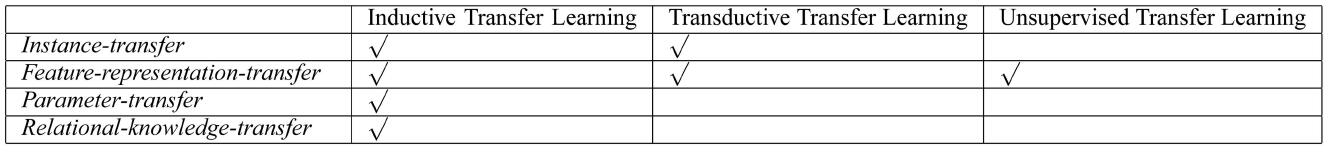
\includegraphics[width=40pc]{img/survey_tab3.jpg}
\end{table*}

\begin{figure*}[!ht]
\centering
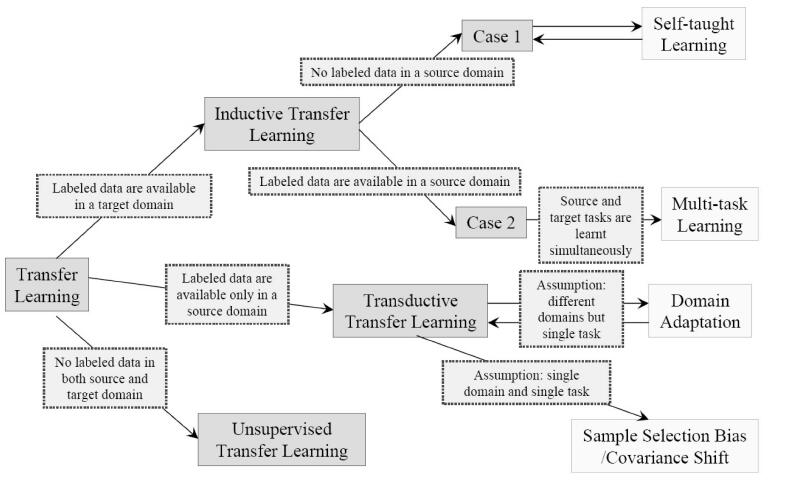
\includegraphics[width=30pc]{img/survey_fig1.jpg}
\caption{迁移学习方法与情境的关系}
\label{fig:survey_method}
\end{figure*}


\begin{enumerate}
\item 在归纳迁移的情境中, 目标任务和源任务是不同的, 而目标域和源域可能相同也可能不同. 此类问题中, 目标域中必须要有带标签的数据才能训练出目标预测模型$f_T(\cdot)$. 根据源域中无标签数据和标签数据的情形不同, 我们还能进一步将归纳迁移算法分为这样两类:\\
a. 源域中有很多标签数据. 此时归纳迁移算法类似于多任务学习算法. 但区别在于, 前者更侧重于在目标问题中取得更好的性能, 而后者则试图同时完成源任务和目标任务. \\
b. 源域中无标签数据. 此时归纳学习算法比较接近自学(self-taught learning)算法. 因为在自学算法的使用场景中源任务和目标任务的标签空间可能不同, 而这与源域中无标签数据的情形是很近似的. 

\item 在转导学习的情境中, 目标任务和源任务是一样的, 但源域和目标域是不同的. 这种情况下目标域是没有标签数据的, 但源域有很多. 根据源域和目标域之间的区别, 我们还能进一步将转到学习的情境划分为这样两类:\\
a. 二者的特征空间不同$X_S \ne X_T$\\
b. 特征空间相同$X_S \ne X_T$, 但边缘概率分布不同, $P(X_S) \ne P(X_T)$\\
后者和文本分类中的域适应很相似, 因为他们的基本假设是一样的. 
\item 最后, 还有无监督迁移学习的情境. 它与归纳迁移学习的情境类似, 目标问题和源问题不同但相关. 区别在于, 无监督迁移学习中目标问题是无监督问题, 如聚类、降维等. 在此情境中, 源域和目标域都没有带标签的数据. 
\end{enumerate}




\section{结论}

地下城与勇士没有妹子好玩. 

\bibliographystyle{IEEEtran}
\bibliography{thesis}

\end{document}
